%\documentclass[10pt,xcolor=svgnames]{beamer} %Beamer  % This is Wrong! Please do not consider
\documentclass[10pt,svgnames]{beamer} %Beamer
\usepackage{palatino} %font type
\usefonttheme{metropolis} %Type of slides
\usefonttheme[onlymath]{serif} %font type Mathematical expressions
\usetheme[progressbar=frametitle,titleformat frame=smallcaps,numbering=counter]{metropolis} %This adds a bar at the beginning of each section.
\useoutertheme[subsection=false]{miniframes} %Circles in the top of each frame, showing the slide of each section you are at

\usepackage{appendixnumberbeamer} %enumerate each slide without counting the appendix
\setbeamercolor{progress bar}{fg=Maroon!70!Coral} %These are the colours of the progress bar. Notice that the names used are the svgnames
\setbeamercolor{title separator}{fg=DarkSalmon} %This is the line colour in the title slide
\setbeamercolor{structure}{fg=black} %Colour of the text of structure, numbers, items, blah. Not the big text.
\setbeamercolor{normal text}{fg=black!87} %Colour of normal text
\setbeamercolor{alerted text}{fg=DarkRed!60!Gainsboro} %Color of the alert box
\setbeamercolor{example text}{fg=Maroon!70!Coral} %Colour of the Example block text

\setbeamercolor{palette primary}{bg=NavyBlue!50!DarkOliveGreen, fg=white} %These are the colours of the background. Being this the main combination and so one. 
\setbeamercolor{palette secondary}{bg=NavyBlue!50!DarkOliveGreen, fg=white}
\setbeamercolor{palette tertiary}{bg=NavyBlue!40!Black, fg= white}
\setbeamercolor{section in toc}{fg=NavyBlue!40!Black} %Color of the text in the table of contents (toc)

% =========================
%   Added Packages
% =========================
\usepackage{natbib}



%These next packages are the useful for Physics in general, you can add the extras here. 
\usepackage{amsmath,amssymb}
\usepackage{slashed}
\usepackage{cite}
\usepackage{relsize}
\usepackage{caption}
\usepackage{subcaption}
\usepackage{multicol}
\usepackage{booktabs}
\usepackage[scale=2]{ccicons}
\usepackage{pgfplots}
\usepgfplotslibrary{dateplot}
\usepackage{geometry}
\usepackage{xspace}
\newcommand{\themename}{\textbf{\textsc{bluetemp}\xspace}}%metropolis}}\xspace}

\title{Perbedaan Pria dan Wanita \citep{susabda2021konseling}}
\author[Name]{Hendra Bunyamin} %With inst, you can change the institution they belong
\subtitle{Renungan Komsel}
%\institute[uni]{\inst{$\dagger$} Department of blah blah \\ University of \LaTeX}
\date{\today} %Here you can change the date
\titlegraphic{\vspace{-0.5cm}\hfill
\includegraphics[scale=0.23]{images/logo-gkia-komit.png}} %You can modify the location of the logo by changing the command \vspace{}. 

\begin{document}
{
\setbeamercolor{background canvas}{bg=NavyBlue!50!DarkOliveGreen, fg=white}
\setbeamercolor{normal text}{fg=white}
\maketitle
}%This is the colour of the first slide. bg= background and fg=foreground

\metroset{titleformat frame=smallcaps} %This changes the titles for small caps

%\begin{frame}{The Bunyamins}
%	\centering
%	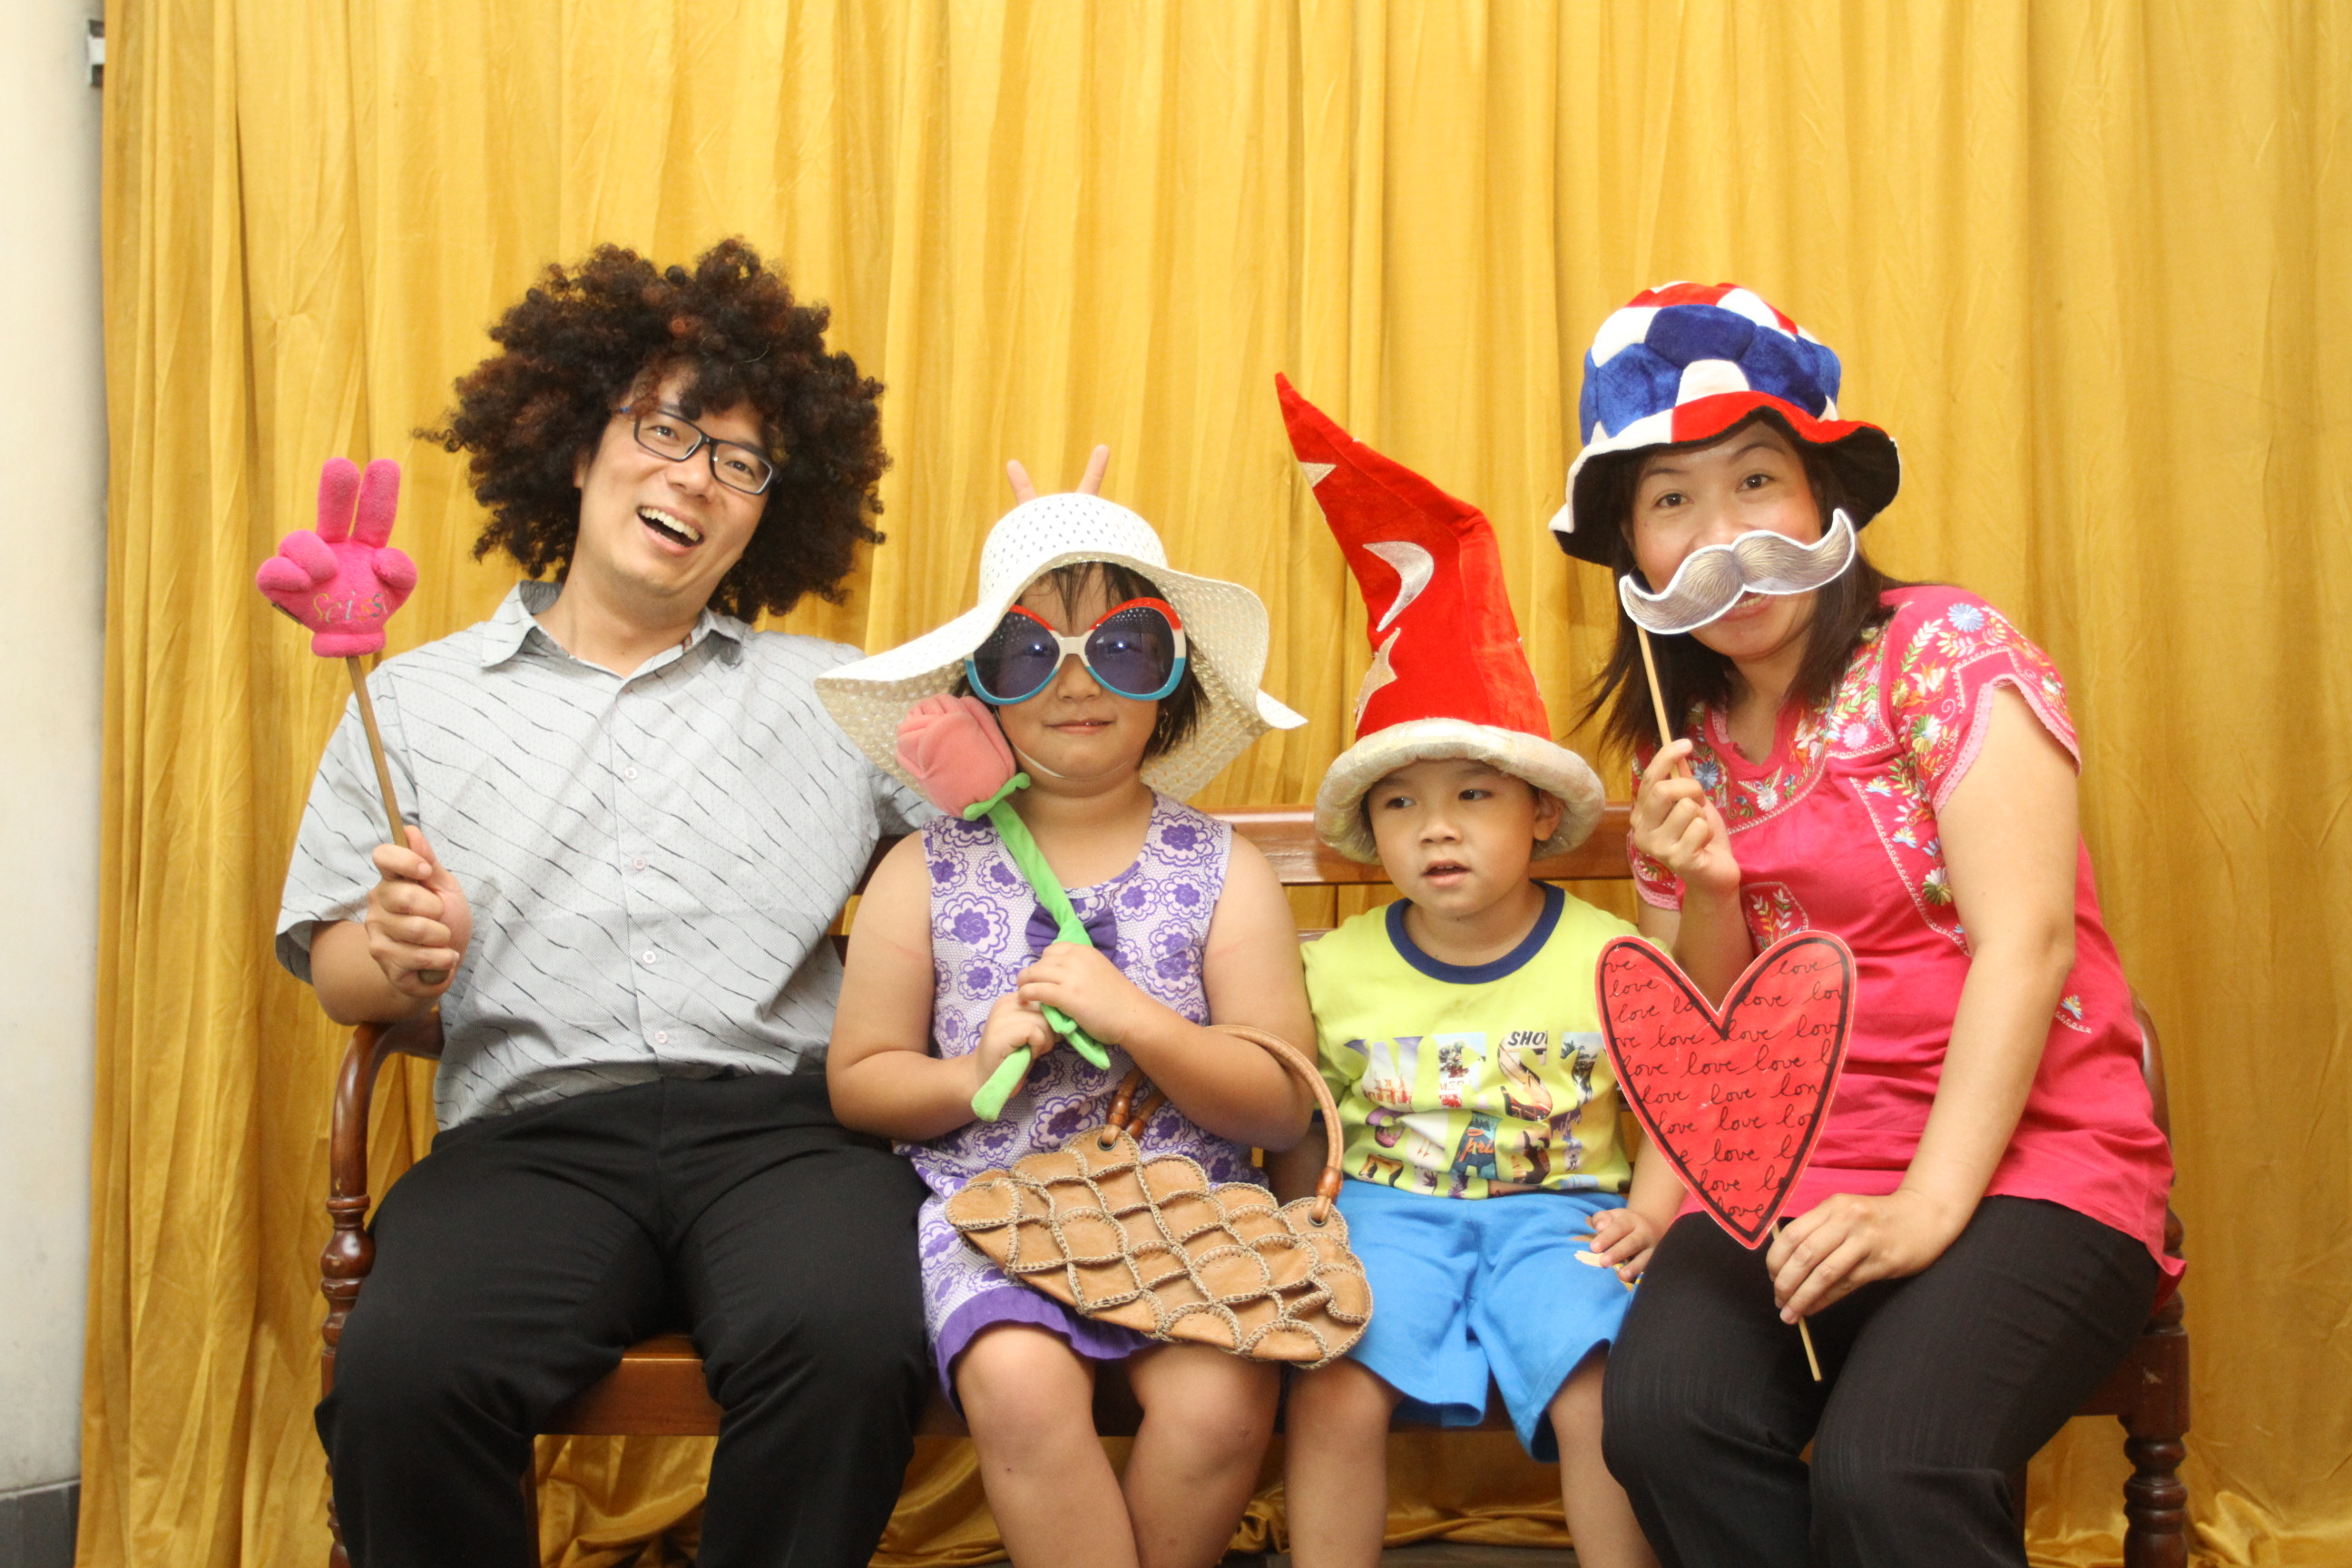
\includegraphics[scale=.12]{images/family-gullit}
%\end{frame}

\begin{frame}{Outline}
  \setbeamertemplate{section in toc}[sections numbered] %This is numbering the sections
  \tableofcontents[hideallsubsections] %You can comment this line if you want to show the subsections in the table of contents
\end{frame}

\section{Apa Kata Alkitab?}
\begin{frame}{Apa kata Alkitab? (1/7)}
 	\emph{Pembacaan Alkitab}
	\begin{itemize}
		\item<2-> \textbf{Kejadian 2:18 (TB)}\\
		\onslide<3-> TUHAN Allah berfirman: "\textit{Tidak baik, kalau manusia itu seorang diri saja. Aku akan menjadikan penolong baginya, yang sepadan dengan dia.}"
	\end{itemize}
	
	\begin{center} 
		\includegraphics<4->[scale=.22]{images/my-other-half}
	\end{center}
\end{frame}

\begin{frame}{Apa kata Alkitab? (2/7)}
 	\emph{Pembacaan Alkitab}
	\begin{itemize}
		\item<2-> \textbf{Kejadian 2:18 (BIMK)}\\
		\onslide<3-> Lalu Tuhan Allah berkata, "\textit{Tidak baik manusia hidup sendirian. Aku akan membuat teman yang cocok untuk membantunya.}"
	\end{itemize}
	
	\begin{center} 
		\includegraphics<4->[scale=.11]{images/team-work}
	\end{center}
\end{frame}

\begin{frame}{Apa kata Alkitab? (3/7)}
	\begin{center} 
		\includegraphics<1->[scale=.08]{images/cowboy-alone-desert} 
	\end{center}	
\end{frame}

\begin{frame}{Apa kata Alkitab? (4/7)}
 	\emph{Pembacaan Alkitab}
	\begin{itemize}
		\item<2-> \textbf{Efesus 5:21-23 (TSI)} \\
		\onslide<3-> \textit{Wujud menghormati Kristus dalam hubungan dengan sesama}
				
		\bigskip
		\onslide<4-> Hendaklah kamu rendah hati dan bersedia menghormati kemauan satu sama lain. \onslide<5-> Dengan begitu kamu juga menghormati Kristus. 
		
		\bigskip
		\onslide<6-> \textit{Dalam hubungan suami-istri} 
		
		\bigskip
		\onslide<7-> Jika kamu seorang istri, hendaklah kamu menaati suamimu sama seperti menaati Tuhan Yesus. \onslide<8-> Karena suami adalah kepala dari istri, sama seperti Kristus adalah kepala dari seluruh jemaat Allah. \onslide<9->Sebagai tubuh Kristus, kita taat kepada Dia yang sudah menyelamatkan kita.
	\end{itemize}
%		\includegraphics<5->[scale=.235]{images/natural-order-in-a-family}	
\end{frame}

\begin{frame}{Apa kata Alkitab? (5/7)}
 	\emph{Pembacaan Alkitab}
	\begin{itemize}				
		\item<2-> \textbf{Efesus 5:25, 28 (BIMK)} \\
		\onslide<3-> Suami, kasihilah istrimu, sama seperti Kristus mengasihi jemaat serta mengurbankan diri-Nya untuk jemaat itu. 
		
		\bigskip
		\onslide<4-> Begitulah juga suami harus mengasihi istrinya seperti ia mengasihi tubuhnya sendiri. \onslide<5->Orang yang mengasihi istrinya berarti ia mengasihi dirinya sendiri. 
	\end{itemize}
%		\includegraphics<5->[scale=.235]{images/natural-order-in-a-family}	
\end{frame}

\begin{frame}{Apa kata Alkitab? (6/7)}
 	\emph{Pembacaan Alkitab}
	\begin{itemize}
		\item<2-> \textbf{Kolose 3:18-19 (BIMK)} \\
		\onslide<3-> \textit{Hubungan-hubungan pribadi dalam hidup yang baru}
				
		\bigskip
		
		\onslide<4-> Saudara-saudara yang menjadi istri! \onslide<5->Taatlah kepada suamimu, sebab begitulah seharusnya kelakuanmu sebagai orang Kristen. 
		
		\bigskip
		\onslide<6->Saudara-saudara yang menjadi suami! \onslide<7->Kasihilah istrimu. Jangan kasar terhadap mereka.
	\end{itemize}
%		\includegraphics<5->[scale=.235]{images/natural-order-in-a-family}	
\end{frame}

\begin{frame}{Apa kata Alkitab? (7/7)}
 	\emph{Pembacaan Alkitab}
	\begin{itemize}
		\item<2-> \textbf{1 Petrus 3:1-2, 7 (BIMK)}: \textit{Suami dan isteri} \\
		\onslide<3-> Begitu juga kalian, istri-istri, harus tunduk kepada suami supaya kalau di antara mereka ada yang tidak percaya kepada berita dari Allah, kelakuanmu dapat membuat mereka menjadi percaya. \onslide<4-> Dan tidak perlu kalian mengatakan apa-apa kepada mereka,sebab mereka melihat kelakuanmu yang murni dan saleh.

		\bigskip
		\onslide<5-> Dan kalian juga, suami-suami, hendaklah hidup dengan penuh pengertian terhadap istrimu, dan dengan kesadaran bahwa mereka adalah kaum yang lemah. \onslide<6-> Perlakukanlah mereka dengan hormat, sebab mereka bersama-sama dengan kalian, akan menerima anugerah hidup yang sejati dari Allah. \onslide<7->Lakukanlah ini, supaya tidak ada yang menghalangi doamu. 
	\end{itemize}
%		\includegraphics<5->[scale=.235]{images/natural-order-in-a-family}	
\end{frame}


\section{Natural Order of the Family}
\begin{frame}{Natural Order of the Family}
	\begin{columns}
	\begin{column}{0.5\textwidth}
	\begin{center}
		\includegraphics<1->[width=1\textwidth]{images/natural-order-in-a-family}
	\end{center}			
	\end{column}	
	\begin{column}{0.5\textwidth}
		Husband $\rightarrow$ 
		\begin{itemize}
			\item<2-> Spiritually lead the family 
			\item<3-> Provide for the family
			\item<4-> Love wife like Christ loves the church
		\end{itemize}				
		Wife $\rightarrow$ 
		\begin{itemize}
			\item<5-> Be a helper to her husband
			\item<6-> Raise Godly Children
			\item<7-> Submit to husband's authority
		\end{itemize}						
	\end{column}
	\end{columns}		
\end{frame}

\section{Natur Pria dan Wanita}
\begin{frame}{Natur berbeda antara pria dan wanita}
	    \textbf{Kejadian 3:16-19}
	    \begin{itemize}
	    	\item<2-> "\textit{Susah payahmu waktu mengandung akan Kubuat sangat banyak; dengan kesakitan engkau akan melahirkan anakmu ...}". \\
	    	\onslide<3-> $\Longrightarrow$ Wanita mendapatkan pemuasan batinnya melalui kesakitan pada saat ia melahirkan anaknya.
	    	\item<4-> "\textit{... engkau akan berahi kepada suamimu dan ia akan berkuasa atasmu.}". \\
	    	\onslide<5-> $\Longrightarrow$ Ketergantungan wanita pada suaminya. \\
	    	\item<6-> "\textit{... terkutuklah tanah karena engkau; dengan bersusah payah engkau akan mencari rezekimu dari tanah seumur hidupmu: ...}" \\
	    	\onslide<7-> $\Longrightarrow$ Pria mengelola bumi dan mendapatkan makanan melalui tenaga yang diperasnya (\textit{lebih membutuhkan kekuatan fisik}).
	    \end{itemize}
%Firman-Nya kepada perempuan itu: "\textit{Susah payahmu waktu mengandung akan Kubuat sangat banyak; dengan kesakitan engkau akan melahirkan anakmu; namun engkau akan berahi kepada suamimu dan ia akan berkuasa atasmu.}" ......, maka \textit{terkutuklah tanah karena engkau; dengan bersusah payah engkau akan mencari rezekimu dari tanah seumur hidupmu: semak duri dan rumput duri yang akan dihasilkannya bagimu, dan tumbuh-tumbuhan di padang akan menjadi makananmu; dengan berpeluh engkau akan mencari makananmu, sampai engkau kembali lagi menjadi tanah, karena dari situlah engkau diambil; sebab engkau debu dan engkau akan kembali menjadi debu.}"
\end{frame}

\section{Tokoh Alkitab I}
\begin{frame}{Natur berbeda antara pria dan wanita (1/4)}
\begin{figure}[!ht]
	\centering
	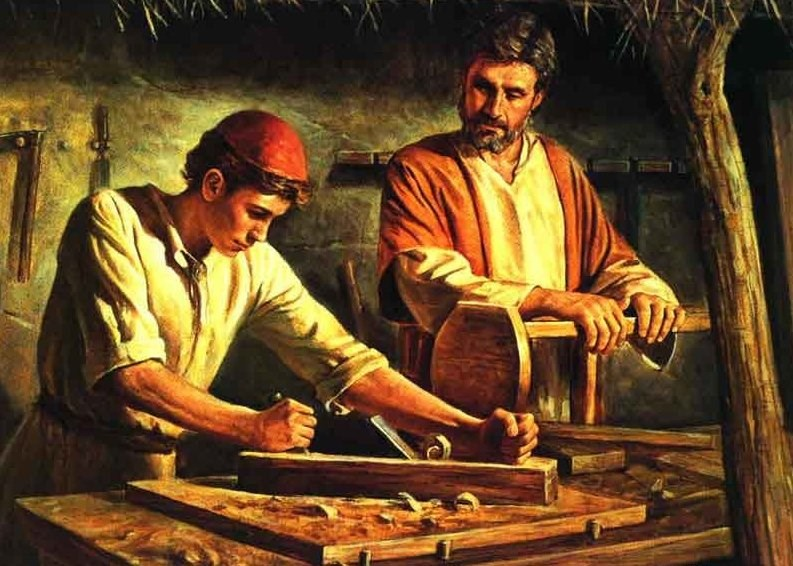
\includegraphics[scale=.5]{images/joseph-father} 		
	\caption{\only<2->{Yusuf, ayah Tuhan Yesus \citep{studyresources1992menwomen}}}
\end{figure}	
\end{frame}

\begin{frame}{Natur berbeda antara pria dan wanita (2/4)}
\emph{Yusuf} (\textbf{Matius 1:18-20}): 

	\onslide<2-> Karena Yusuf suaminya, \textit{seorang yang tulus hati dan tidak mau mencemarkan nama isterinya di muka umum, ia bermaksud menceraikannya dengan diam-diam}.
	
	\bigskip
	\onslide<3-> $\Longrightarrow$ Natur yang \textit{yang lebih rasional, cenderung menyelesaikan masalah secara praktis}.

%Kelahiran Yesus Kristus adalah seperti berikut: Pada waktu Maria, ibu-Nya, bertunangan dengan Yusuf, ternyata ia mengandung dari Roh Kudus, sebelum mereka hidup sebagai suami isteri. Karena Yusuf suaminya, \textit{seorang yang tulus hati dan tidak mau mencemarkan nama isterinya di muka umum, ia bermaksud menceraikannya dengan diam-diam}. Tetapi ketika ia mempertimbangkan maksud itu, malaikat Tuhan nampak kepadanya dalam mimpi dan berkata: "Yusuf, anak Daud, janganlah engkau takut mengambil Maria sebagai isterimu, sebab anak yang di dalam kandungannya adalah dari Roh Kudus. 		
\end{frame}

\begin{frame}{Natur berbeda antara pria dan wanita (3/4)}
\begin{figure}[!ht]
	\centering
	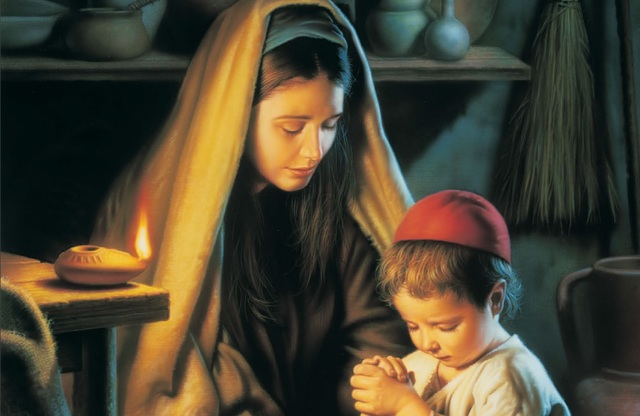
\includegraphics[scale=.5]{images/mary-mother} 		
	\caption{\only<2->{Maria, ibu Tuhan Yesus \citep{beckstrom2015national}}}
\end{figure}	
\end{frame}

\begin{frame}{Natur berbeda antara pria dan wanita (4/4)}
\emph{Maria} (\textbf{Lukas 1:46-54}): \\
	\onslide<2-> "\textit{Jiwaku memuliakan Tuhan, dan hatiku bergembira karena Allah, Juruselamatku ... Sesungguhnya, mulai dari sekarang segala keturunan akan menyebut aku berbahagia}"
	
	\bigskip
	\onslide<3-> $\Longrightarrow$ Maria bereaksi secara \textit{emosional} atas berita sukacita yang malaikat sampaikan kepadanya.
%Lalu kata Maria: "Jiwaku memuliakan Tuhan, dan hatiku bergembira karena Allah, Juruselamatku sebab Ia telah memperhatikan kerendahan hamba-Nya. Sesungguhnya, mulai dari sekarang segala keturunan akan menyebut aku berbahagia, karena Yang Mahakuasa telah melakukan perbuatan-perbuatan besar kepadaku dan nama-Nya adalah kudus. ......" 	
\end{frame}

\begin{frame}{Menti Time I}
	\begin{enumerate}
		\item Go to \texttt{www.menti.com}
		\item Use the code \texttt{8377 1355}
	\end{enumerate}
\end{frame}


\section{Tokoh Alkitab II}
\begin{frame}{Natur berbeda antara pria dan wanita (1/7)}
\begin{figure}[!ht]
	\centering
	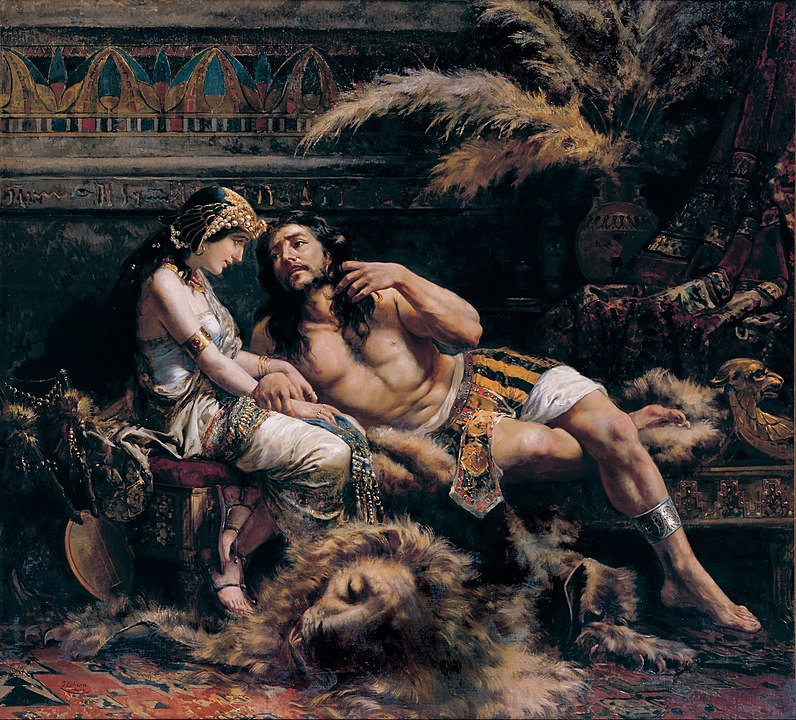
\includegraphics[scale=.275]{images/samson-and-delilah} 		
	\caption{\only<2->{Samson dan Delilah \citep{errazquin1887samson}}}
\end{figure}	
\end{frame}

\begin{frame}{Natur berbeda antara pria dan wanita (2/7)}
	\textbf{Dalam pemenuhan dan pelampiasan kebutuhan seksual}
	
	\bigskip
	\onslide<2-> \emph{Samson} (\textbf{Hakim-Hakim 14-16}):
\begin{itemize}
	\item<3-> "\textit{Di Timna aku melihat seorang gadis Filistin. Tolong, ambillah dia menjadi isteriku.}"
	\item<4-> "\textit{Ambillah dia bagiku, sebab dia kusukai.}"
	\item<5-> \textit{Sesudah itu Simson jatuh cinta kepada seorang perempuan dari lembah Sorek yang namanya Delila}.
\end{itemize}
%	Ia pulang dan memberitahukan kepada ayahnya dan ibunya: "Di Timna aku melihat seorang gadis Filistin. Tolong, ambillah dia menjadi isteriku. Tetapi ayahnya dan ibunya berkata kepadanya: "Tidak adakah di antara anak-anak perempuan sanak saudaramu atau di antara seluruh bangsa kita seorang perempuan, sehingga engkau pergi mengambil isteri dari orang Filistin, orang-orang yang tidak bersunat itu?" Tetapi jawab Simson kepada ayahnya: "Ambillah dia bagiku, sebab dia kusukai." \\
%	$\cdots$ \\
%		$\cdots$ \\
%			$\cdots$ \\
%	Sesudah itu Simson jatuh cinta kepada seorang perempuan dari lembah Sorek yang namanya Delila.
\end{frame}

\begin{frame}{Natur berbeda antara pria dan wanita (3/7)}
\begin{figure}[!ht]
	\centering
	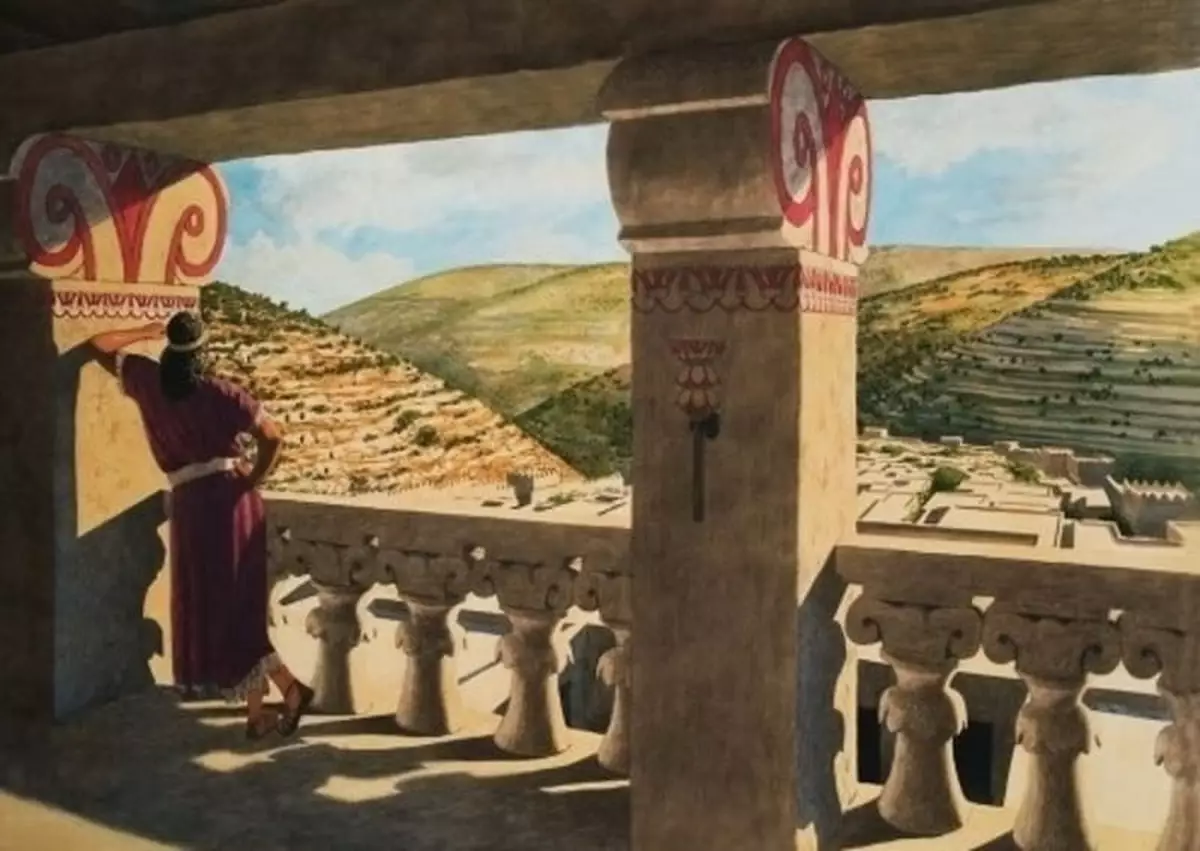
\includegraphics[scale=.23]{images/bathsheba} 		
	\caption{\only<2->{Daud dan Batsyeba \citep{biblestudy2016david}}}
\end{figure}	
\end{frame}

\begin{frame}{Natur berbeda antara pria dan wanita (4/7)}
	\emph{Daud} \textbf{(2 Samuel 11)}: 
	\begin{itemize}
		\item<2-> "\textit{...tampak kepadanya dari atas sotoh itu seorang perempuan sedang mandi; perempuan itu sangat elok rupanya.}" 
		\item<3-> \textit{Sesudah itu Daud menyuruh orang mengambil dia}.
		\item<4-> lalu \textit{Daud tidur dengan dia}.
	\end{itemize}		
%	...... Sekali peristiwa pada waktu petang, ketika Daud bangun dari tempat pembaringannya, lalu berjalan-jalan di atas sotoh istana, tampak kepadanya dari atas sotoh itu seorang perempuan sedang mandi; perempuan itu sangat elok rupanya. Lalu Daud menyuruh orang bertanya tentang perempuan itu dan orang berkata: "Itu adalah Batsyeba binti Eliam, isteri Uria orang Het itu." Sesudah itu Daud menyuruh orang mengambil dia. Perempuan itu datang kepadanya, lalu \textit{Daud tidur dengan dia}. Perempuan itu baru selesai membersihkan diri dari kenajisannya. Kemudian pulanglah perempuan itu ke rumahnya.	
\end{frame}

\begin{frame}{Natur berbeda antara pria dan wanita (5/7)}
\begin{figure}[!ht]
	\centering
	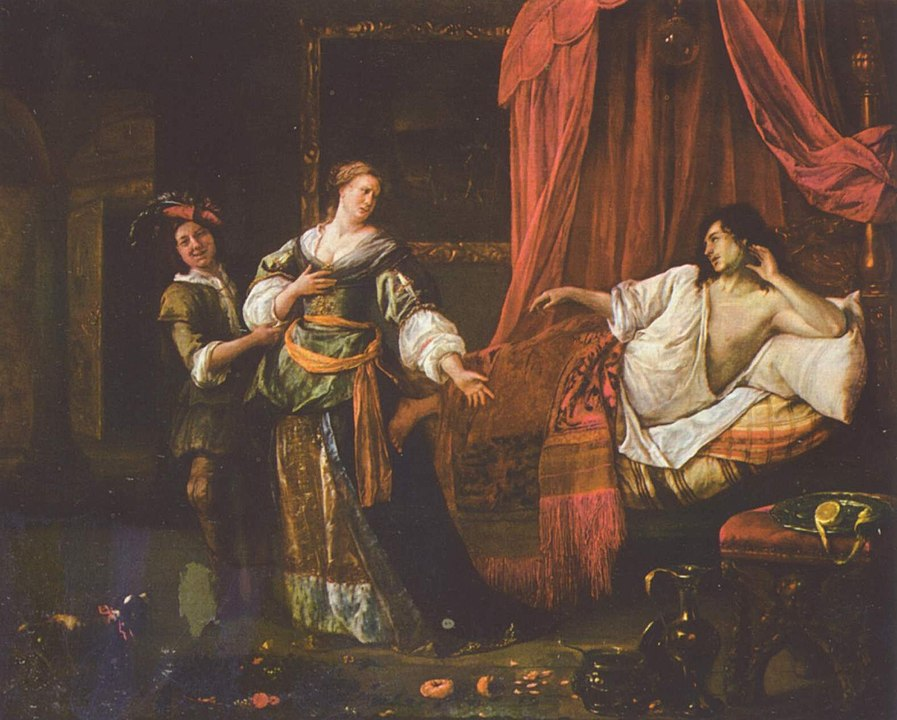
\includegraphics[scale=.275]{images/amnon-dan-tamar}     		
	\caption{\only<2->{Amnon dan Tamar \citep{steen1661amnon}}}
\end{figure}	
\end{frame}

\begin{frame}{Natur berbeda antara pria dan wanita (6/7)}
	\emph{Amnon} \textbf{(2 Samuel 13)}:  
	\begin{itemize}
		\item<2-> Absalom bin Daud mempunyai seorang adik perempuan yang cantik, namanya Tamar.
		\item<3-> Hati Amnon sangat tergoda, sehingga ia pura-pura jatuh sakit untuk mendapatkan Tamar.
		\item<4-> ... dipegangnyalah gadis itu dan berkata kepadanya: "\textit{Marilah tidur dengan aku, adikku}."
		\item<5-> Tetapi Amnon tidak mau mendengarkan perkataannya, dan \textit{sebab ia lebih kuat dari padanya, diperkosanyalah dia}, lalu tidur dengan dia.
	\end{itemize}		
\end{frame}

\begin{frame}{Natur berbeda antara pria dan wanita (7/7)}
		\onslide<2->\textbf{Contoh-Contoh}: Samson, Daud, Amnon 
		
		\bigskip
		\onslide<3-> $\Longrightarrow$ Pria cenderung \textbf{memenuhi dan melampiaskan kebutuhan seksual secara instan dan semata-mata untuk kepuasan instingnya}, sehingga umumnya mereka tidak dapat memisahkan antara cinta dan seks.
\end{frame}


\section{Tokoh Alkitab III}
\begin{frame}{Natur berbeda antara pria dan wanita (1/4)}
\begin{figure}[!ht]
	\centering
	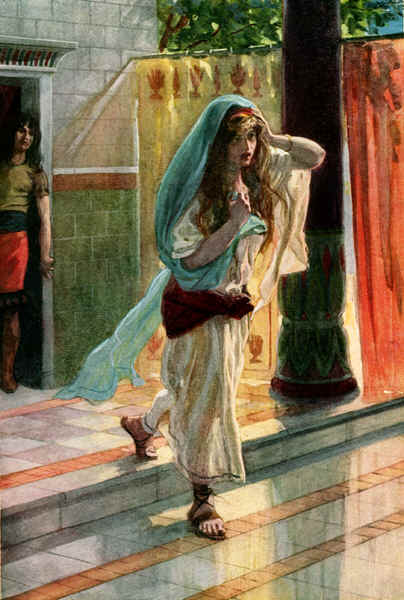
\includegraphics[scale=1]{images/tamar}     		
	\caption{\only<2->{Tamar \citep{riddle2010tamar}}}
\end{figure}	
\end{frame}

\begin{frame}{Natur berbeda antara pria dan wanita (2/4)}
\onslide<2-> \emph{Tamar} \textbf{(2 Samuel 13)}: 
\begin{itemize}
	\item<3-> Lalu Lalu Amnon berkata kepadanya: "\textit{Bangunlah, enyahlah!}". 
	\item<4-> Lalu berkatalah gadis itu kepadanya: "\textit{Tidak kakakku, sebab menyuruh aku pergi adalah lebih jahat dari pada apa yang telah kaulakukan kepadaku tadi.}"
	\item<5-> Lalu Tamar menaruh abu di atas kepalanya, mengoyakkan baju kurung yang maha indah yang dipakainya, meletakkan tangannya di atas kepalanya dan pergilah ia sambil meratap dengan nyaring. 
\end{itemize}
\end{frame}

\begin{frame}{Natur berbeda antara pria dan wanita (3/4)}
\begin{figure}[!ht]
	\centering
	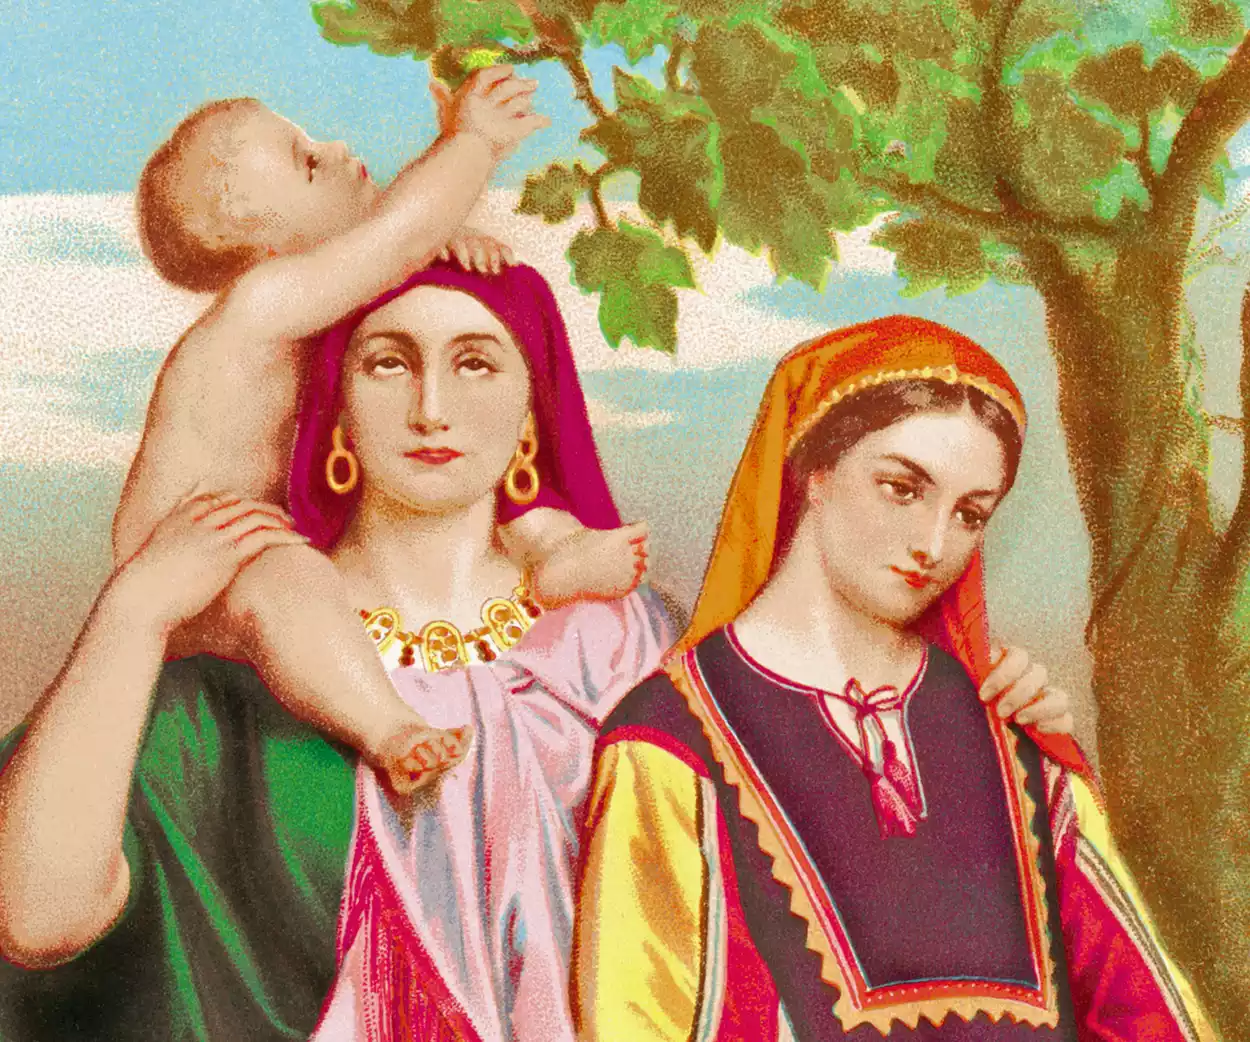
\includegraphics[scale=.175]{images/leah-dan-rachel}     		
	\caption{\only<2->{Lea dan Rahel \citep{zavada2019meetleah}}}
\end{figure}	
\end{frame}

\begin{frame}{Natur berbeda antara pria dan wanita (4/4)}
\onslide<2-> \emph{Lea} \textbf{(Kejadian 30:14-21)}: 

\bigskip
\onslide<3-> Kata Rahel kepada Lea: "\textit{Berilah aku beberapa buah dudaim yang didapat oleh anakmu itu." Jawab Lea kepadanya: "Apakah belum cukup bagimu mengambil suamiku? Sekarang pula mau mengambil lagi buah dudaim anakku?}"

\bigskip

	\onslide<4-> $\Longrightarrow$ \textit{Bagi wanita, hubungan seksual tidak terpisahkan dari keterikatan emosinya}.
	
	\bigskip
	\onslide<5-> $\Longrightarrow$ Hasil empiris juga menemukan bahwa \textit{perzinahan lebih banyak dilakukan oleh pria dibandingkan dengan wanita}. 		
\end{frame}

\begin{frame}{Menti Time II}
	\begin{enumerate}
		\item Go to \texttt{www.menti.com}
		\item Use the code \texttt{89 68 35 1}
	\end{enumerate}
\end{frame}

\begin{frame}{Natur berbeda antara pria dan wanita (1/5)}
\begin{figure}[!ht]
	\centering
	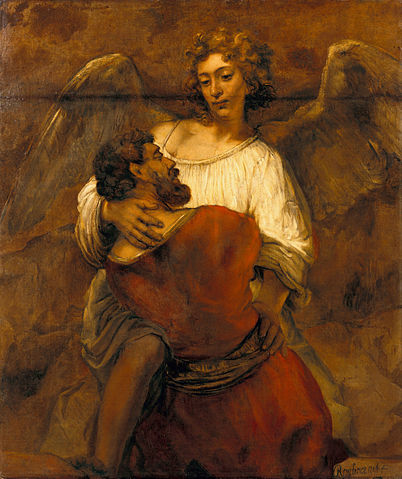
\includegraphics[scale=.4]{images/jacob}     		
	\caption{\only<2->{Yakub bergulat dengan malaikat \citep{rembrandt1659jacob}}}
\end{figure}	
\end{frame}

\begin{frame}{Natur berbeda antara pria dan wanita (2/5)}
	\textbf{Dalam orientasi hidup}
	
	\bigskip
	\onslide<2-> \emph{Yakub} \textbf{(Kejadian 29)}:
	\begin{itemize}
		\item<3-> Yakub cinta kepada Rahel, sebab itu ia berkata: "\textit{Aku mau bekerja padamu tujuh tahun lamanya untuk mendapat Rahel, anakmu yang lebih muda itu.}"
		\item<4-> Jadi bekerjalah Yakub tujuh tahun lamanya untuk mendapat Rahel itu, tetapi yang tujuh tahun itu dianggapnya seperti beberapa hari saja, karena cintanya kepada Rahel. 
		\item<5-> "\textit{... kemudian anakku yang lainpun akan diberikan kepadamu sebagai upah, asal engkau bekerja pula padaku tujuh tahun lagi}".
		\item<6-> Demikianlah ia bekerja pula pada Laban tujuh tahun lagi.
	\end{itemize}			
\end{frame}

\begin{frame}{Natur berbeda antara pria dan wanita (3/5)}
\begin{figure}[!ht]
	\centering
	\includegraphics[scale=.175]{images/rich-young-man}     		
	\caption{\only<2->{Kristus dan pemuda yang kaya \citep{hofmann1889rich}}}
\end{figure}	
\end{frame}


\begin{frame}{Natur berbeda antara pria dan wanita (4/5)}
\emph{Pemuda yang kaya} \textbf{(Matius 19)}: 
\begin{itemize}
	\item<2-> Kata orang muda itu kepada-Nya: "\textit{Semuanya itu telah kuturuti, apa lagi yang masih kurang?}"
	\item<3-> Kata Yesus kepadanya: "\textit{Jikalau engkau hendak sempurna, pergilah, juallah segala milikmu dan berikanlah itu kepada orang-orang miskin, maka engkau akan beroleh harta di sorga, kemudian datanglah ke mari dan ikutlah Aku.}"
	\item<4-> Ketika orang muda itu mendengar perkataan itu, pergilah ia dengan sedih, sebab banyak hartanya.
\end{itemize}
\end{frame}

\begin{frame}{Natur berbeda antara pria dan wanita (5/5)}
	
	\textbf{Contoh}: Yakub dan pemuda yang kaya.

	\bigskip
	\onslide<2-> $\Rightarrow$ Pria lebih cenderung \textit{memiliki orientasi hidup pada target dan upaya pencapaiannya} (\textit{target-oriented}). 

\end{frame}

\begin{frame}{Natur berbeda antara pria dan wanita (1/5)}
\begin{figure}[!ht]
	\centering
	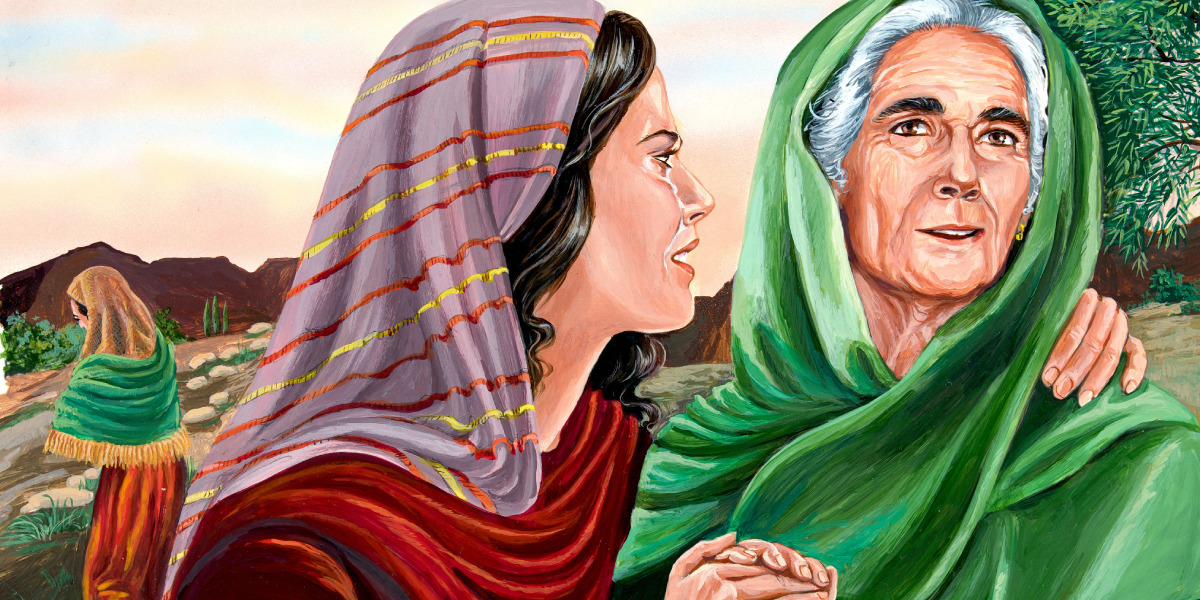
\includegraphics[scale=.25]{images/ruth-and-naomi}     		
	\caption{\only<2->{Rut dan Naomi \citep{jehovah2021ruth}}}
\end{figure}	
\end{frame}

\begin{frame}{Natur berbeda antara pria dan wanita (2/5)}
	\emph{Rut} \textbf{(Rut 1:16-17)}:  

	\bigskip	
	\onslide<2-> Tetapi kata Rut: "\textit{... di mana engkau mati, akupun mati di sana, dan di sanalah aku dikuburkan.}"	
\end{frame}

\begin{frame}{Natur berbeda antara pria dan wanita (3/5)}
\begin{figure}[!ht]
	\centering
	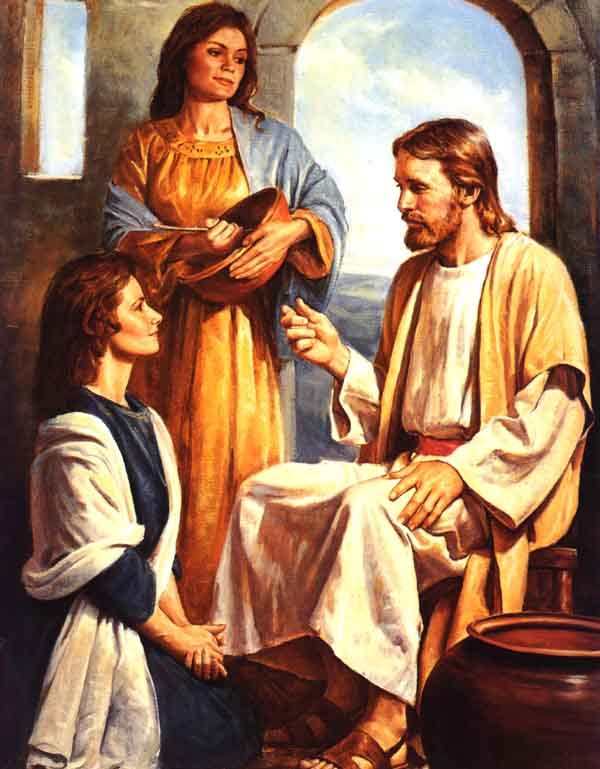
\includegraphics[scale=.4]{images/mary-and-martha}     		
	\caption{\only<2->{Kristus bersama Maria dan Martha \citep{bible2021mary}}}
\end{figure}	
\end{frame}

\begin{frame}{Natur berbeda antara pria dan wanita (4/5)}
	\emph{Maria saudara Lazarus} \textbf{(Yohanes 12:1-8)}: 

	\bigskip	
	\onslide<2-> ... \textit{Maka Maria mengambil setengah kati minyak narwastu murni yang mahal harganya, lalu meminyaki kaki Yesus dan menyekanya dengan rambutnya; dan bau minyak semerbak di seluruh rumah itu.}
\end{frame}

\begin{frame}{Natur berbeda antara pria dan wanita (5/5)}
	\begin{itemize}
		\item<2-> \textbf{Orientasi wanita berubah pada saat kesempatan membina hubungan pribadi itu terbuka} (\textit{relational-oriented}).
		
		\bigskip		
		
		\onslide<3-> \textbf{Contoh}: Rut dan Maria saudara Lazarus (Yohanes 12:1-8).		
	\end{itemize}
\end{frame}

\begin{frame}{Menti Time III}
	\begin{enumerate}
		\item Go to \texttt{www.menti.com}
		\item Use the code \texttt{4274 2105}
	\end{enumerate}
\end{frame}


\section{Kesimpulan}
\begin{frame}{Kesimpulan}
	\begin{columns}
	\begin{column}{0.5\textwidth}
	\begin{center}
		\includegraphics<1->[width=1\textwidth]{images/natural-order-in-a-family}
	\end{center}			
	\end{column}	
	\begin{column}{0.5\textwidth}
		Husband $\rightarrow$ 
		\begin{itemize}
			\item<2-> Spiritually lead the family 
			\item<3-> Provide for the family
			\item<4-> Love wife like Christ loves the church
		\end{itemize}				
		Wife $\rightarrow$ 
		\begin{itemize}
			\item<5-> Be a helper to her husband
			\item<6-> Raise Godly Children
			\item<7-> Submit to husband's authority
		\end{itemize}						
	\end{column}
	\end{columns}		
\end{frame}




%\begin{frame}{Objectives}
%\underline{\textsc{Some text:}}
%\begin{small}
%This is some small Text. 
%\end{small}
%
%\metroset{block=fill}
%\begin{exampleblock}{\textsc{Example block}}
%\begin{itemize}
%    \item You know how to do itemize
%    \item Also here
%\end{itemize}
%\end{exampleblock}
%\end{frame}


%\section{Introduction}
%
%\begin{frame}[fragile]{Introduction: blah blah} %You can change fragile by standout
%Text Text Text Text. \\You can change the size of the footnote text like  Text\footnote{\small{ here.}} Text\footnote{\large{And here.}} Text\footnote{\tiny{And here.}}
%\begin{itemize} %The symbol of the items can be changed by which ever you want, this is just an example.
%    \item[$\diamond$] Text,
%    \item[$\diamond$] Text,
%    \item[$\diamond$] Text.
%\end{itemize}
%An equation without number could be represented by:
%\begin{equation*}
%    c^{2} = a^{2} + b^{2}
%\end{equation*}
%That's all for this slide.
%\end{frame}
%
%\begin{frame}[standout]{This is other type of slide}
%There is some text here.
%And an equation with number:
%\begin{equation}
%    E^{2} = m^{2} + p^{2}
%\end{equation}
%\end{frame}
%
%\section[Outsider section]{Exotic section}

\begin{frame}{Hello}
    You can actually include a new section outside and edit apart.
\end{frame}
%
%\section{This is another section}
%\begin{frame}{Frame Title} %You can also not write fragile or standout and you can see how it looks
%    Hello world!
%\end{frame}
%
%\section{Final section}
%
%\begin{frame}{Conclusion}
%    These are the final words, you do your best to try to wake up everyone that was listening to your talk.
%\end{frame}
%

%{\setbeamercolor{palette primary}{fg=black, bg=white!30} %You can change the colours
%\begin{frame}[standout]
%%  Thank you! And thank to yourself because you did all the job. 
%		\centering
\includegraphics[scale=1]{images/thank-you}	
%		hendra.bunyamin@it.maranatha.edu
%\end{frame}
%}
%
%\begin{frame}[plain]
%		\centering
\includegraphics[scale=1]{images/thank-you}	
%		hendra.bunyamin@gmail.com
%\end{frame}


\appendix
\begin{frame}[allowframebreaks]
  \frametitle<presentation>{}
    {\footnotesize
    \bibliographystyle{apalike}
    \bibliography{references}
    }    
\end{frame}

%\begin{frame}{Back up}
%    These slides won't appear in the table of contents and will not be counted as the total slides.
%\end{frame}
{\setbeamercolor{palette primary}{fg=black, bg=white!30} %You can change the colours
\begin{frame}[standout]
%  Thank you! And thank to yourself because you did all the job. 
		\centering
\includegraphics[scale=1]{images/thank-you}	
		hendra.bunyamin@it.maranatha.edu
\end{frame}
}



\end{document}
